\documentclass{book}

\usepackage[latexmk,mathjax,HomeHTMLFilename=index]{lwarp}
\CSSFilename{style.css}
\MathJaxFilename{javascript.txt}
\setcounter{FileDepth}{1}
\setcounter{tocdepth}{1}
\boolfalse{CombineHigherDepths}

\usepackage{amsmath,amssymb}
\usepackage{lipsum}
\usepackage{tikz}
\usepackage{hyperref}
\usepackage{siunitx}

\input{lwarp-filename-maker.tex} % name files after the short section names in brackets

\begin{document}

\title{Test of Latex to html with lwarp, potentially for my masters thesis}
\author{Paul Lobpreis}

\HTMLTitle{Example}
\HTMLTitleAfterSection
%%%%%%%%%%%%%%%%%%%%%%%%%%%%%%%%%%%%%%%%%%%%%%%%%%%%%%
\maketitle

\label{table-of-contents}

\tableofcontents

%%%%%%%%%%%%%%%%%%%%%%%%%%%%%%%%%%%%%%%%%%%%%%%%%%%%%%
\section[index]{Introduction}

% The titlepage

\BlockClassSingle{manual-title-block}{%
\BlockClassSingle{manual-title}{Hier der Titel der Arbeit}
\BlockClassSingle{manual-version}{Version 1}
}

\lipsum[1-3]
%%%%%%%%%%%%%%%%%%%%%%%%%%%%%%%%%%%%%%%%%%%%%%%%%%%%%%

\chapter[chapter1]{Chapter 1}
\section[section1]{Section 1}
\lipsum[1-3]

\subsection{Introduction}
\lipsum[1-3]

Mathematics:
\[
    \int_0^1 x^2 \, dx = \frac{1}{3}    
\]

\subsection{Details}
\lipsum[4]

%%%%%%%%%%%%%%%%%%%%%%%%%%%%%%%%%%%%%%%%%%%%%%%%%%%%%%
\begin{tikzpicture}
%%%%%%%%%%%%%%%%%%%%%%%%%%%%%%%%%%%%%%%%%%%%%%%%%%%%%%
	\draw[fill=orange](0,0) circle (2cm);
%%%%%%%%%%%%%%%%%%%%%%%%%%%%%%%%%%%%%%%%%%%%%%%%%%%%%%
\end{tikzpicture}
%%%%%%%%%%%%%%%%%%%%%%%%%%%%%%%%%%%%%%%%%%%%%%%%%%%%%%



\section[section2]{Section 2}
\lipsum[4-7]







\chapter[chapter2]{Chapter 2}
\section[section3]{sonstwas}


\chapter[theory]{theory}
\section[section3]{nochwas}
\section{Imaging with fast electrons}

The development of EM has had a profound impact on the field of materials science, enabling researchers to gain insights into the atomic and nanoscale structures of materials, and to comprehend their composition, defects, and functionalities.
Over the past few decades, electron microscopy has undergone significant advancements.
The techniques that were previously reliant upon photographic film now employ high-end cameras and direct electron detectors.
\par This facilitates the capture of increasingly large datasets and allows for a detailed analysis of the structure and composition of a multitude of materials.
The capture of increasingly large datasets thus enables a detailed interpretation of the structure and composition of a multitude of materials.
These developments in EM have been paralleled by advancements in computational power, which have provided researchers with access to powerful computational resources capable of handling the data-intensive requirements of modern microscopy.
In the current era, the rapid evolution of artificial intelligence and machine learning has enabled scientists to analyze extensive data and also to apply complex algorithms to extract meaningful insights from them.
This symbiotic progress between EM and computing has accelerated materials research, thereby opening new avenues for discovery.

\par At the core of EM effectiveness lies the strong interaction between fast electrons and matter compared to photons.
In a Transmission Electron Microscope (TEM), a focused electron beam is directed through a thin sample, typically less than \SI{100}{\nano\metre} thick.
As the electrons pass through the sample, they interact with the matter in various ways, as illustrated in Figure \ref{fig:electronww}.
These interactions result in a variety of signals, which can be captured by different detectors and provide insights into the material properties.

%%%%%%%%%%%%%%%%%%%%%%%%%%%%%%
\begin{figure}[ht]
    \centering
    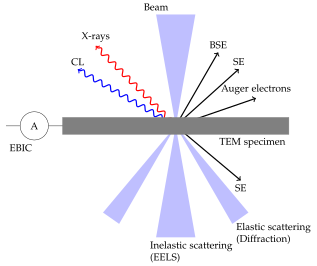
\includegraphics[width=0.65\textwidth]{Introduction/figures/electronww.pdf}
    \caption[Schematic representation of different electron-specimen interactions]{Schematic representation of different electron-specimen interactions of a thin specimen, including inelastic and elastic scattering, X-rays, cathodoluminescence, backscattered and secondary electrons, Auger electrons, and electron beam-induced current}
    \label{fig:electronww}
\end{figure}
%%%%%%%%%%%%%%%%%%%%%%%%%%%%%%


\section{Modes of Transmission electron microscopy}

A Transmission electron microscope (TEM) system consists of an electron gun/illumination system for the generation of electrons and transportation to the sample, electromagnetic lenses to focus during image formation, and detectors for image capturing. 
These components enable different imaging modes, primarily conventional TEM and scanning TEM (STEM), each with bright-field (BF) and dark-field (DF) options.
\par In bright-field transmission electron microscopy (BF-TEM), the aperture is positioned to focus on the unscattered (direct) electron beam. 
In this mode, regions that exhibit a strong scattering effect appear darker, as these regions divert electrons from their original trajectory.
In DF-TEM, an aperture is positioned around a diffracted beam, respectively tilting the beam such that a diffracted beam is on-axis, making regions that scatter electrons in that direction appear bright in the image.
\par In contrast to TEM, STEM employs a scanning approach, whereby a focused and convergent electron beam is scanned across the sample.
At each scanning point, detectors capture both direct and scattered electrons, resulting in the formation of an image.
Similar to TEM, STEM offers both BF and DF modes, with the imaging characteristics dependent on the detector's position and camera length.

%%%%%%%%%%%%%%%%%%%%%%%%%%%%%%
\begin{figure}[ht]
    \centering
    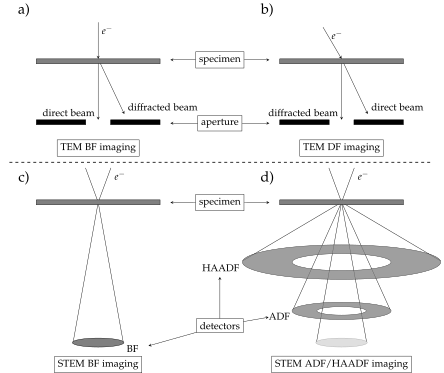
\includegraphics[width=0.85\textwidth]{Introduction/figures/TEM_modi.pdf}
    \caption[Comparison of of BF and DF imaging in TEM and STEM mode]{Comparison of BF and DF imaging in TEM and STEM mode a)  BF imaging in the TEM mode by selecting the unscattered beam through the objective aperture b) DF imaging is obtained by tilting the beam such that a diffracted beam is on-axis c) The on-axis  beam is collected by a BF detector in STEM mode, adjusted to a long camera length compared to DF-STEM d) The annular-dark-field (ADF) and high-angle-annular-dark-field (HAADF) are annular detectors that collect the scattered beam at shorter camera lengths}
    \label{fig:temmodi}
\end{figure}
%%%%%%%%%%%%%%%%%%%%%%%%%%%%%%

Apart from these imaging modes there is a diffraction mode, where the TEM is adjusted to create a diffraction pattern, also known as a reciprocal-space pattern, rather than a real-space image of the sample. 
Here, the electron beam interacts with the crystalline structure of the sample, and the electrons diffract according to Bragg’s law, producing spots or rings that correspond to specific properties of the lattice.
This pattern provides information about the crystal structure, orientation, and strain within the sample. 
Diffraction patterns are formed by focusing on the back focal plane of the objective lens, where the scattering angles of electrons produce a pattern directly related to the atomic structure.




\section{From STEM to 4D-STEM}

The evolution of STEM into 4D-STEM has introduced an even more data-intensive approach to electron microscopy. 
In 4D-STEM, a two-dimensional (2D) array of real space positions is scanned and a 2D diffraction pattern, typically a convergent beam electron diffraction (CBED) is recorded for each of these probe position.

This results in a four-dimensional (4D) dataset...

Figure \ref{fig:4dstem} shows ...


%%%%%%%%%%%%%%%%%%%%%%%%%%%%%%
\begin{figure}[ht]
    \centering
    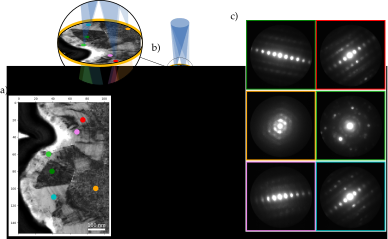
\includegraphics[width=\textwidth]{Introduction/figures/4DSTEM_Overview.pdf}
    \caption[Overview figure of 4D-STEM setup with corresponding CBED patterns]{(a) Simulated real-space image with six marked positions for beam scanning (b) Schematic representation of the 4D-STEM setup, illustrating the scanning beam across the specimen. (c) Corresponding diffraction patterns collected at each marked position, capturing local crystallographic information}
    \label{fig:4dstem}
\end{figure}
%%%%%%%%%%%%%%%%%%%%%%%%%%%%%%

The size of these datasets is substantial. For example, a 4D-STEM scan over a 200 nm x 200 nm area with a 1 nm step size would generate 40,000 scan points. 

\begin{equation}
    \frac{200 \ nm}{1 \ nm} \times \frac{200 \ nm}{1 \ nm} = 40,000 \ \text{scan points}  
\end{equation}

Using a CMOS Camera at 2048 x 2048 pixels with 16-bit resolution, each diffraction pattern occupies approximately \SI{8}{\mega\byte}.

\begin{equation}
    2048 \ \times \ 2048 \ \times \ 2 \ \text{bytes} \approx \SI{8}{\mega\byte}
\end{equation}

This results in a total dataset size of approximately \SI{320}{\giga\byte}, illustrating the data demands of 4D-STEM.

\begin{equation}
    40,000 \ \times \ \SI{8}{\mega\byte} = \SI{320}{\giga\byte}
\end{equation}

To handle such large datasets, researchers often employ several strategies, including increasing the step size, reducing the region of interest (ROI), hardware binning, and utilizing dedicated computing resources for post-processing. 
These computing resources include High-performance computing (HPC) clusters and specialized software, such as py4DSTEM which represent essential tools for managing and analyzing these datasets.



\section{Aim of this work}

The primary aim of this thesis is to conduct 4D-STEM measurements using a FEI Talos F200X equipped with a Gatan Continuum camera, and to process the resulting datasets using the OMNI Cluster at the University of Siegen.
The code used for 4D-STEM processing can be accessed on [link to py4DSTEM GitHub repository], and additional code developed for this thesis is available on [my GitHub repository]. 
Select notebooks/code have also been included in the appendix.




\end{document}

